\documentclass[../../workflow.tex]{subfiles}
\graphicspath{{\subfix{../../img/}}}

\begin{document}

\color{red}
    \begin{enumerate}
        \item There is only one Ih channel gene \parencite{chenFunctionalStudyHyperpolarization2012,gisselmannVariantsDrosophilaMelanogaster2005}
        \item Also known as DMIH (drosophila homologue of HCN channels)
    \end{enumerate}

\color{black}

\section{R5 Model}
\etocignoretoctocdepth % of course, if we want to see something in local TOC...
\etocsettocstyle{\subsection*{\contentsname}}{}
\localtableofcontents

\color{red}
\begin{itemize}
    \item Wang 1994 model simulations
    \begin{itemize}
        \item Blocking T-Type Ca$^{2+}$ channel destroys LTS
        \item Removing h current does not affect dynamics. H current is not
        necessary in the model
    \end{itemize}

    \item Resting membrane potential of R5 is $\approx -49 mV$ \parencite{raccugliaNetworkSpecificSynchronizationElectrical2019}.
\end{itemize}

\color{black}

\subsection{Model}

\newpage
\subsection{Appendix}

\subsubsection{Reverse Engineering Wang 1994 Model}
\begin{figure}[H]
    \centering
    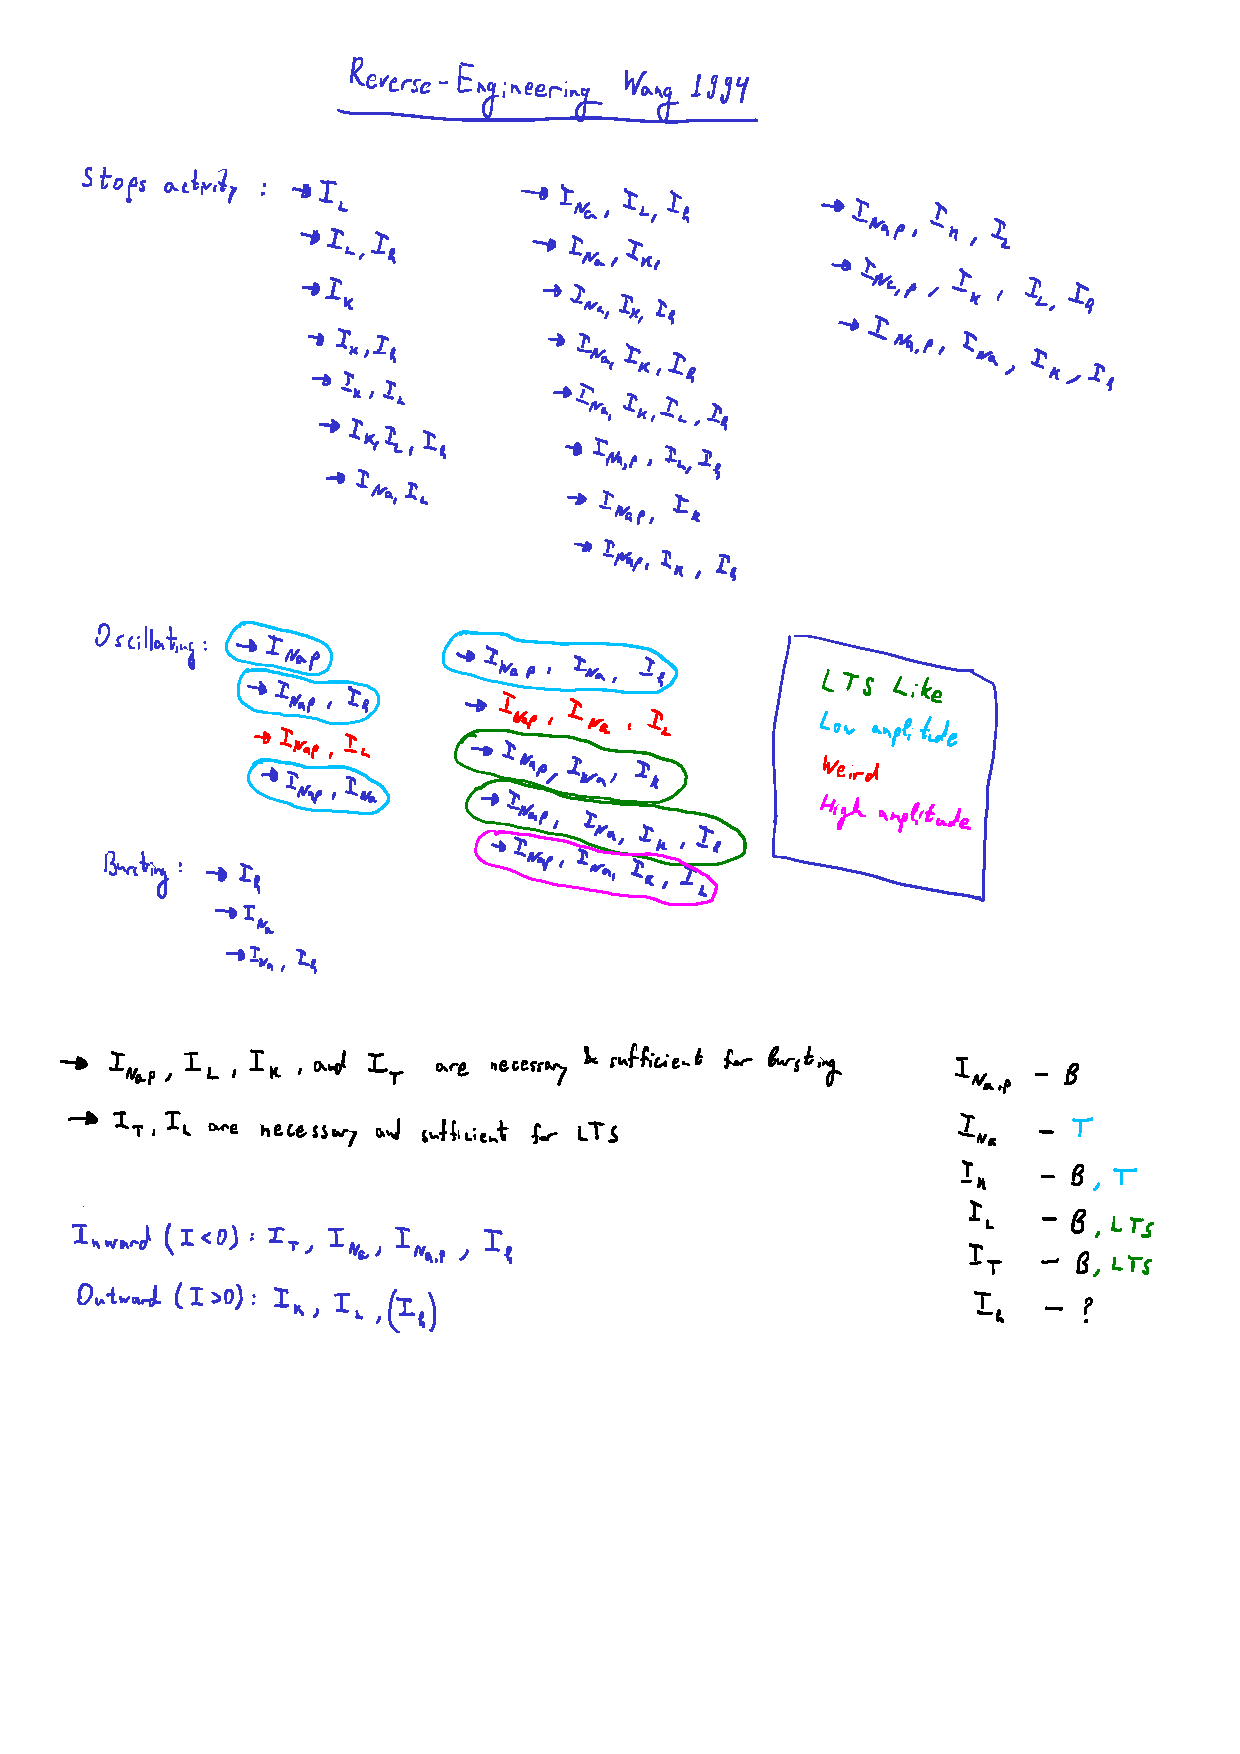
\includegraphics[height=0.9\textheight, page=1]{Handwritten Notes/R5 Model/Wang1994_reverse_engineering.pdf}
\end{figure}

\afterpage{%
    \clearpage
    \begin{figure}[!p]
        \vspace*{\fill} % Add vertical space at the top
        \centering
        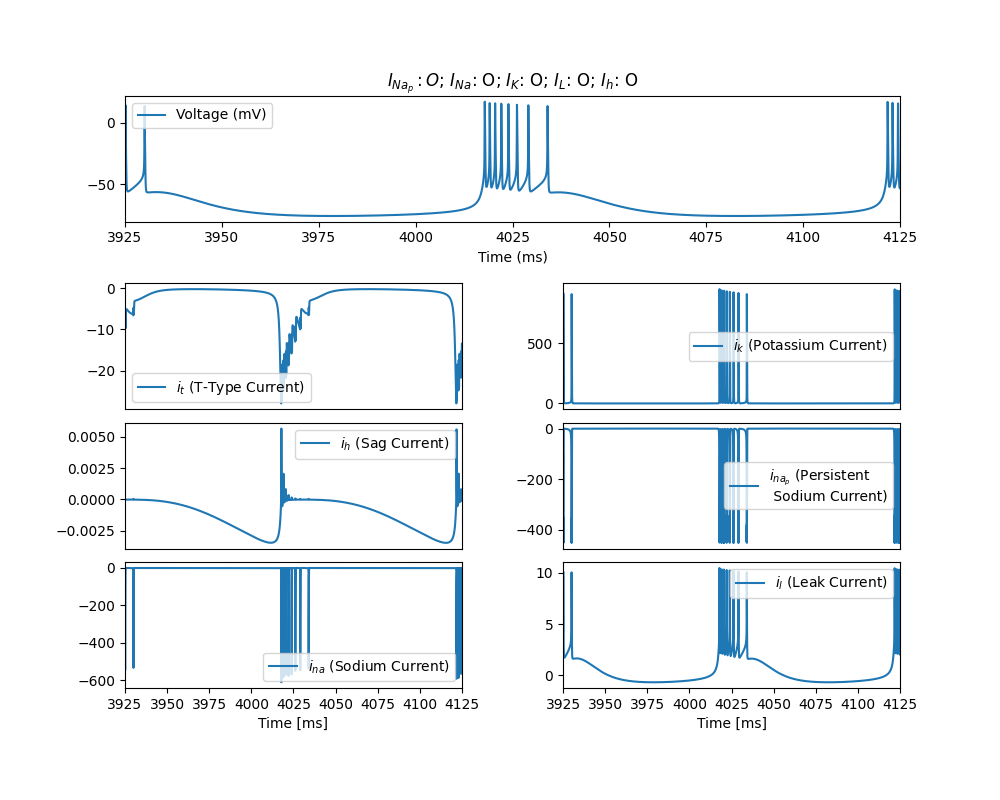
\includegraphics[width=\linewidth]{img/r5/wang1994/currents_experiment_0.png}
        \caption{}
        \vspace*{\fill} % Add vertical space at the bottom
    \end{figure}
    \clearpage
}

\begin{figure}[H]
    \centering
    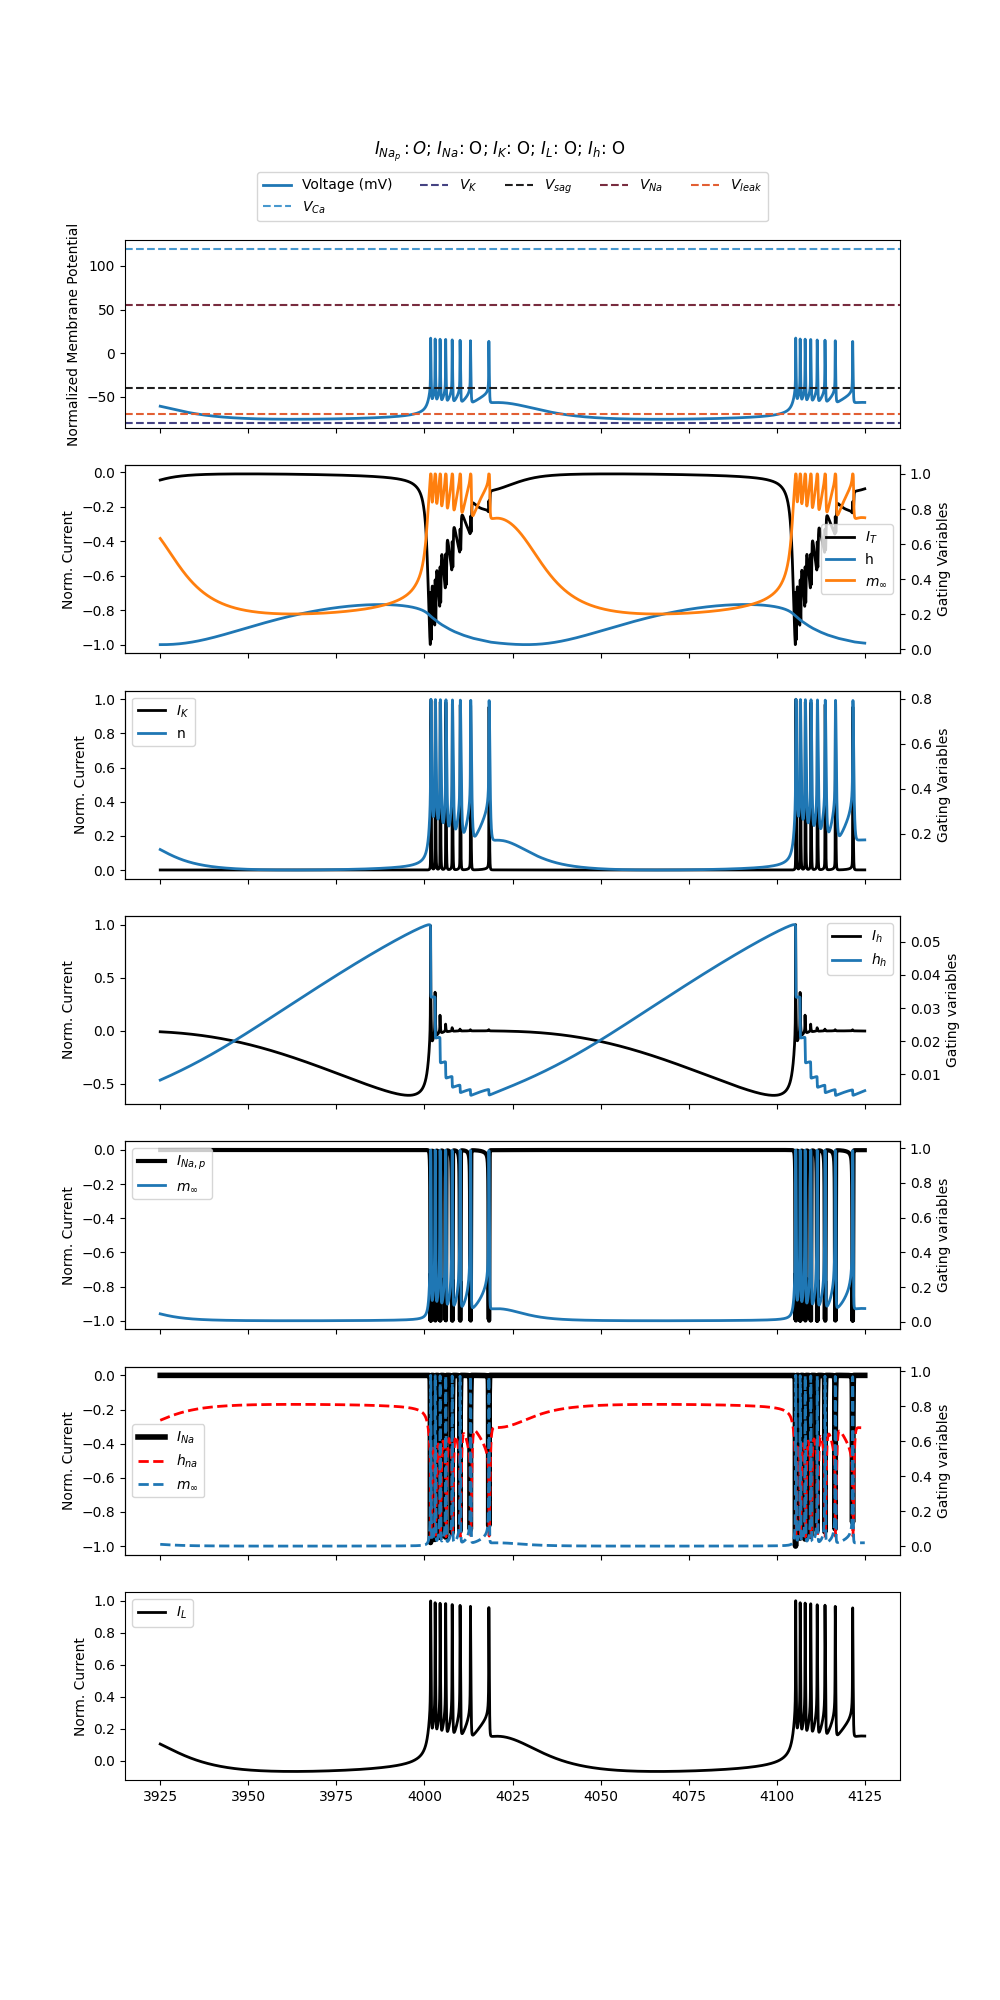
\includegraphics[height=\textheight]{img/r5/wang1994/experiment_0.png}
\end{figure}

\afterpage{%
    \clearpage
    \begin{figure}[!p]
        \vspace*{\fill} % Add vertical space at the top
        \centering
        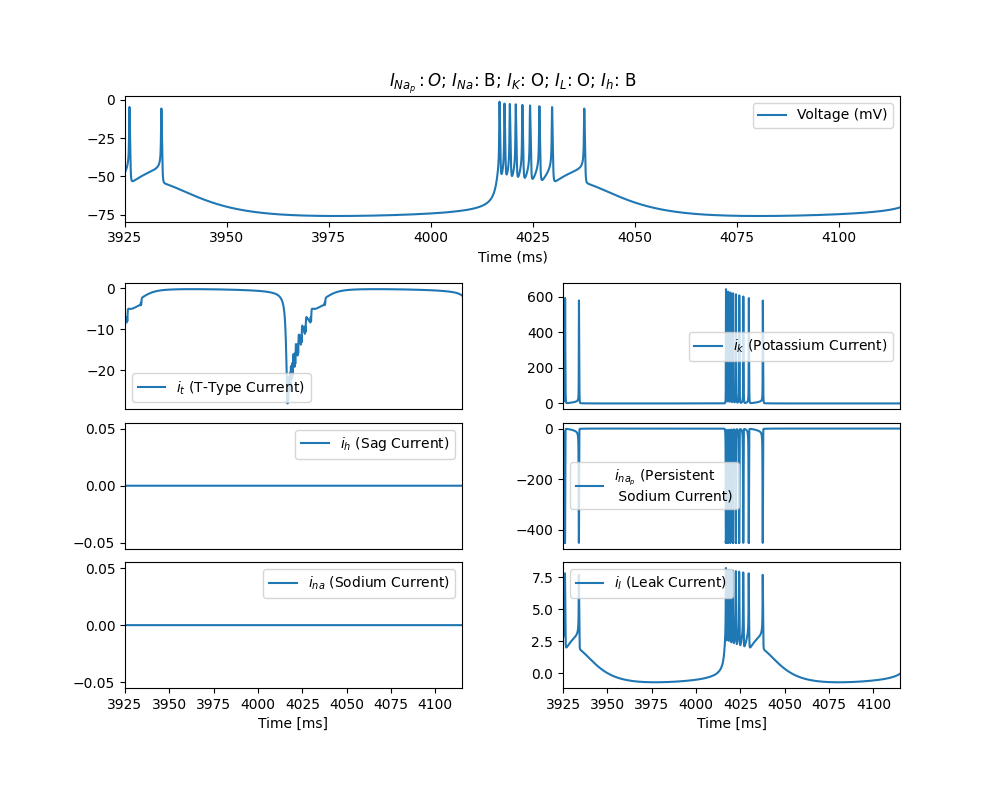
\includegraphics[width=\linewidth]{img/r5/wang1994/currents_experiment_9.png}
        \caption{}
        \vspace*{\fill} % Add vertical space at the bottom
    \end{figure}
    \clearpage
}

\begin{figure}[H]
    \centering
    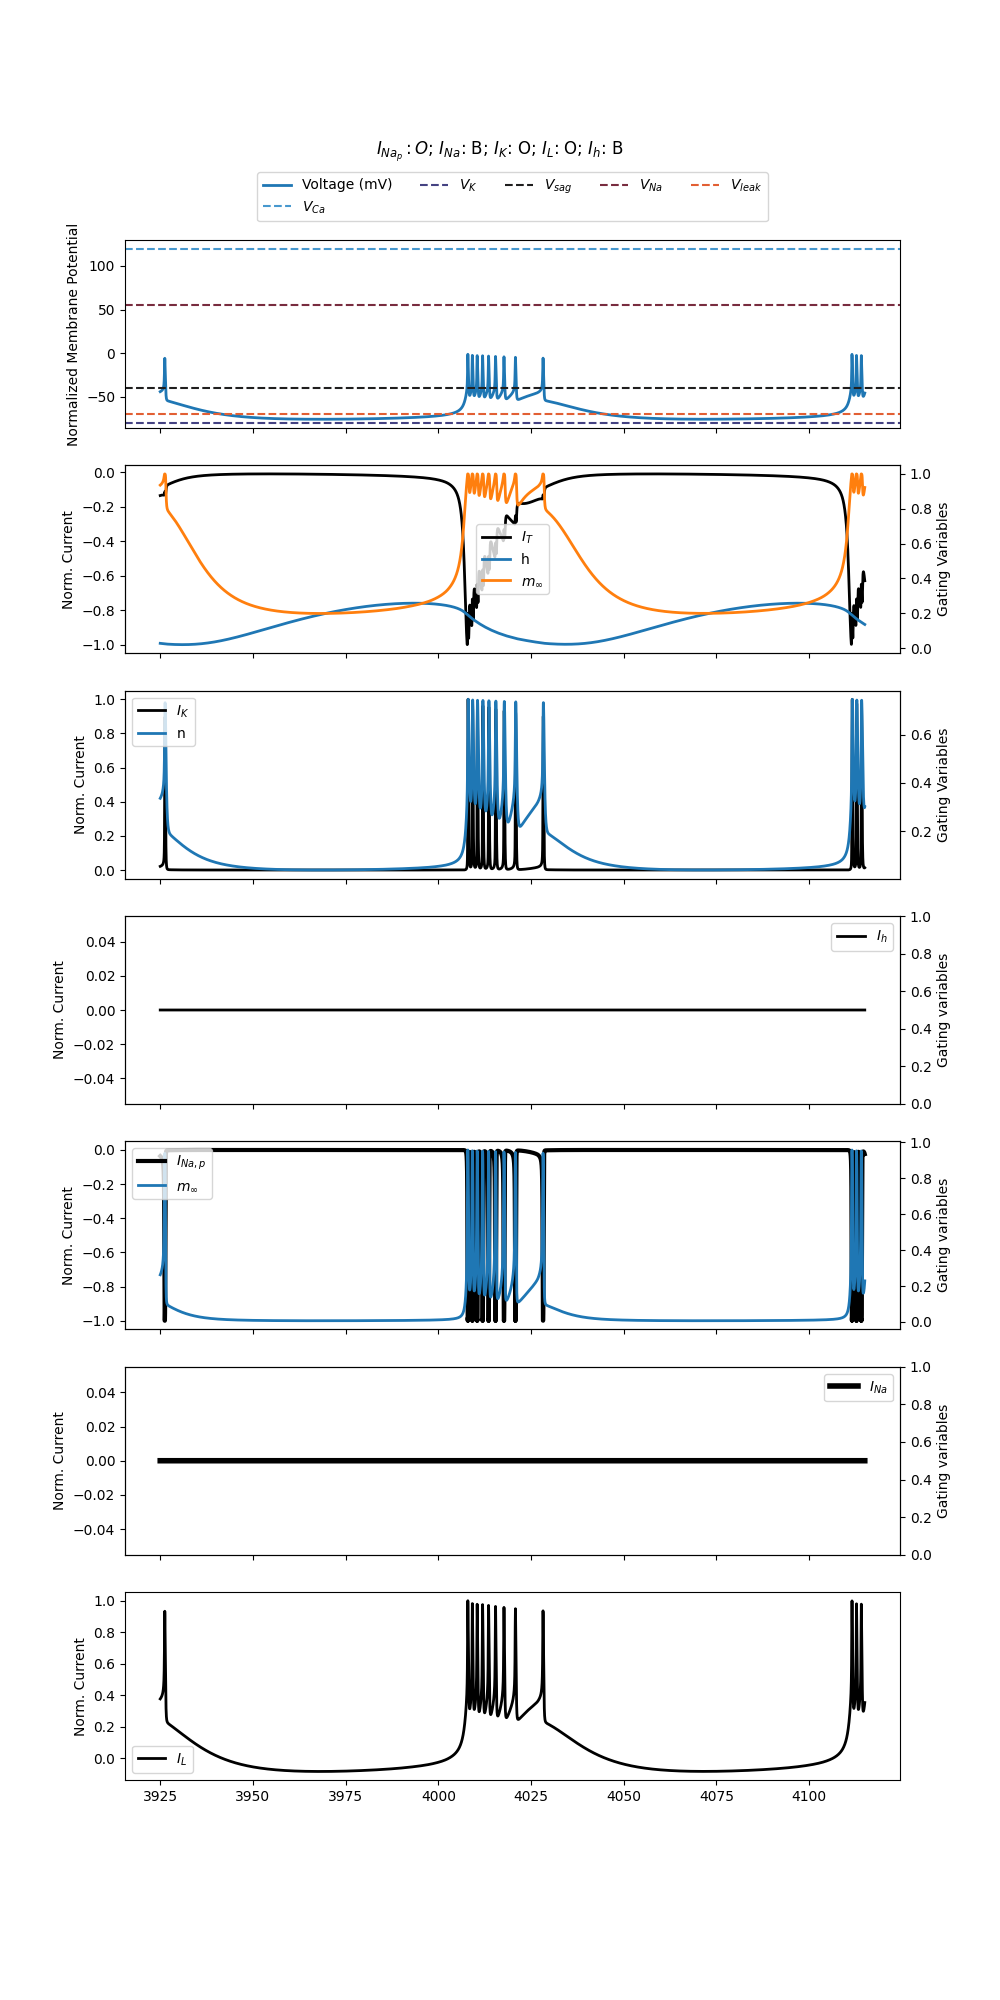
\includegraphics[height=\textheight]{img/r5/wang1994/experiment_9.png}
\end{figure}

\afterpage{%
    \clearpage
    \begin{figure}[!p]
        \vspace*{\fill} % Add vertical space at the top
        \centering
        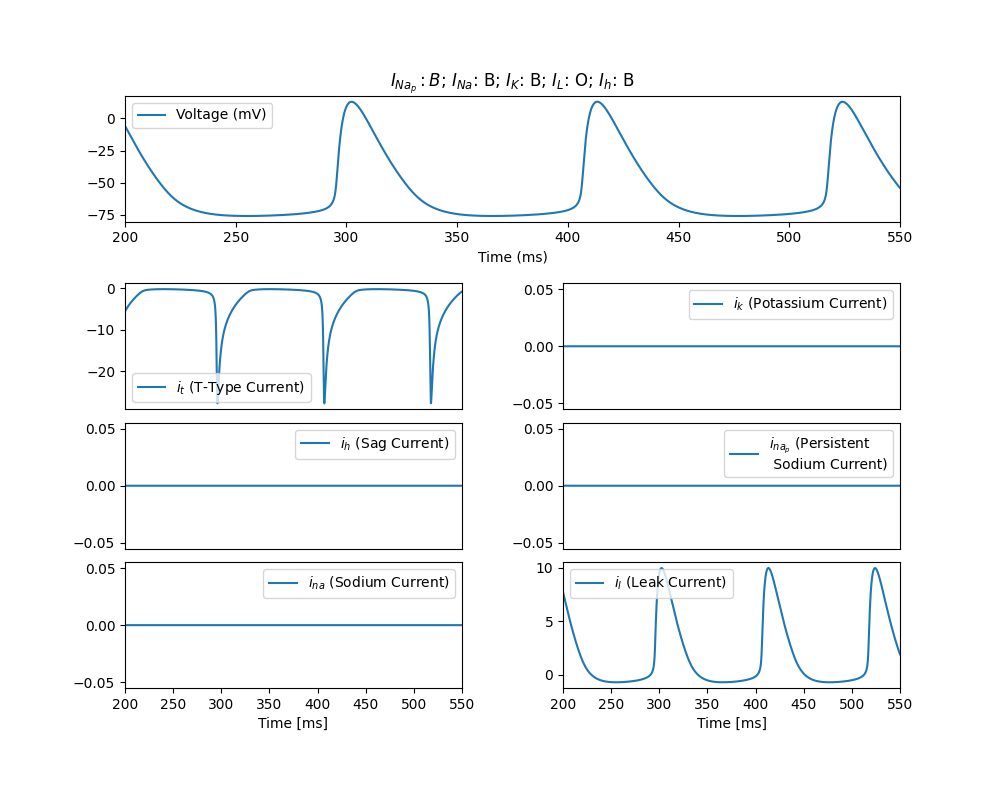
\includegraphics[width=\linewidth]{img/r5/wang1994/currents_experiment_29.png}
        \caption{}
        \vspace*{\fill} % Add vertical space at the bottom
    \end{figure}
    \clearpage
}

\begin{figure}[H]
    \centering
    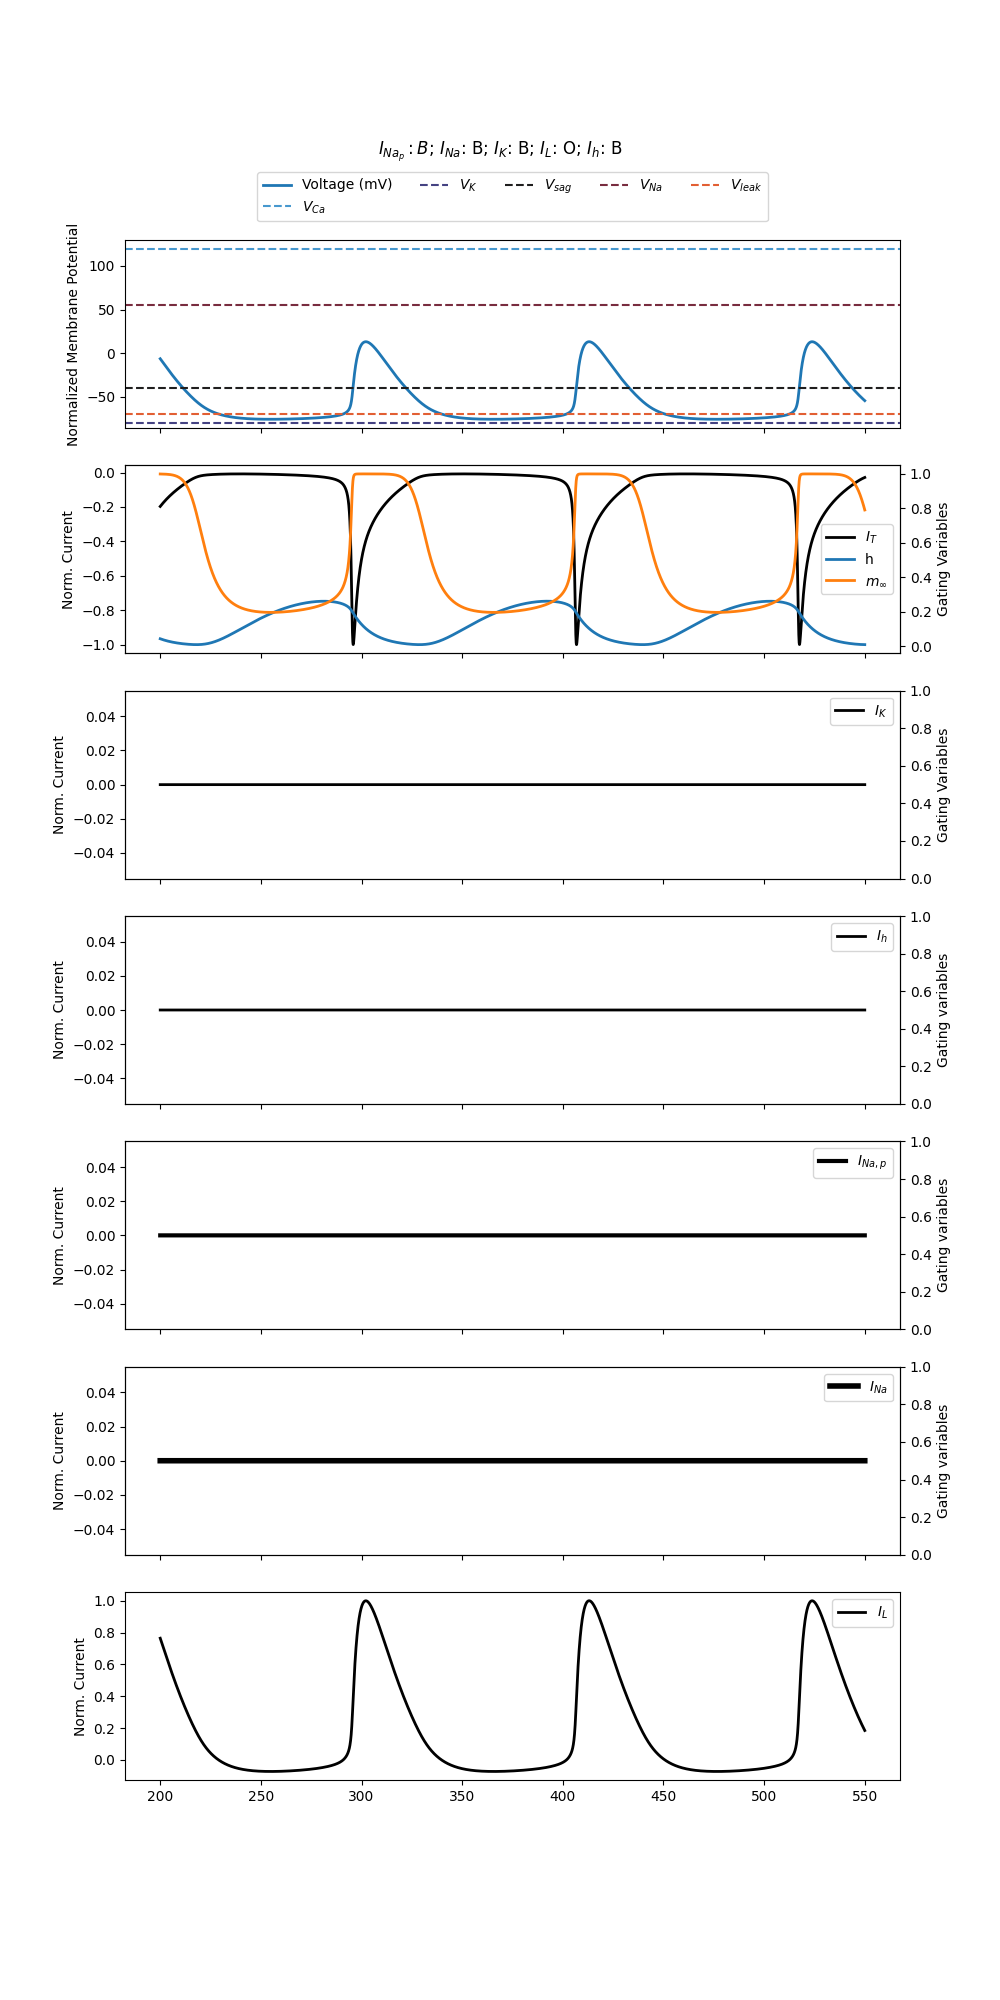
\includegraphics[height=\textheight]{img/r5/wang1994/experiment_29.png}
\end{figure}



\end{document}